% ====================
% Set-Up 
% ====================

% Document class 
\documentclass[11pt,aspectratio=169]{beamer}

% Packages 
\usepackage{pgfpages}
\usepackage{fancyvrb}
\usepackage{tikz}
\usepackage{pgfplots}
\pgfplotsset{compat=newest}
\usepackage{mdframed} %for framed boxes
\usepackage{amsthm} %for theorem formatting 
\usepackage{tcolorbox} % For colored boxes
\usepackage[style=authoryear]{biblatex}

% Custom .sty file 
\usepackage{/Users/posmikdc/Documents/assets/latex/beamer/beamertheme}

% Add bib file  
\addbibresource{main.bib}

% Globals
\input{/Users/posmikdc/Documents/assets/latex/globals}

% ====================
% Title Page 
% ====================

\title{Some Fancy Title: \\ Followed by Some More Title Text}
\titlegraphic{
\includegraphics[width=0.4\textwidth]{img/title}}
\author{\name \inst{1} \and John Doe \inst{2} \and Don Joe \inst{2}}
\institute[shortinst]{\inst{1} \department \\ 
                      \inst{2} Another University, Another Department}  
\date{\today}

\begin{document}

{
  % rather than use the frame options [noframenumbering,plain], we make the
  % color match, so that the indicated page numbers match PDF page numbers
  \setbeamercolor{page number in head/foot}{fg=background canvas.bg}
  \begin{frame}
    \titlepage
  \end{frame}
}

% ====================
% Table of Contents 
% ====================

\begin{frame}{Overview}
    % Throughout your presentation, if you choose to use \section{} and \subsection{} commands, these will automatically be printed on this slide as an overview of your presentation
    \tableofcontents
\end{frame}

% ====================
% Presentation Body  
% ====================

\section{A Major Theme}
\begin{frame}{A slide with footnotes and citations}

A statement referencing \cite{Posmik2022} and with a simple footnote\footnote{Hi, I am a footnote}. 

  \begin{itemize}
    \item Some statement with an in-line citation in parentheses \parencite{Posmik2022} 
    \item Another statement with a short citation in the footnote\footcite{Posmik2022}
    \item A final statement with a long citation in the footnote\footfullcite{Posmik2022} 
	\end{itemize}

	\vspace{3ex}
	\begin{center}
		\scriptsize (a small note)
	\end{center}

\end{frame}

\begin{frame}{A slide title}

  \begin{itemize}
    \item A bulleted item
    \item Another item
      \begin{itemize}
        \item With sub-bullets\footnote{This is also a footnote}
        \item And another, with some \textbf{bold} text
      \end{itemize}
    \item And another, at the top level, with \textit{italic} text
  \end{itemize}

\end{frame}

\section{The Other Major Theme}
\begin{frame}{Theorems, Lemmas, Corollaries, Examples, and Proofs}

\begin{theorem}[The hardest theorem]
We love hard lemmas, $1 + 1 = 2$
\end{theorem}

\begin{lemma}[The hardest lemma]
We love hard lemmas, $1 + 1 = 2$
\end{lemma}

\begin{corollary}[The hardest corollary]
We love hard corollaries, $1 + 1 = 2$
\end{corollary}

\begin{example}[The hardest example]
We love hard examples, $1 + 1 = 2$
\end{example}

\begin{proof}
We love hard proofs, $1 + 1 = 2$
\end{proof}

\end{frame}

\begin{frame}{Blocks of Highlighted Text}
In this slide, some important text will be \alert{highlighted} because it's important. Please, don't abuse it. 



\end{frame}

\begin{frame}{A slide with centered text}

  \begin{center}
    Some statement that is centered.
  \end{center}

  \vspace{2ex}
  \begin{center}
    \scriptsize (a small note)
  \end{center}

\end{frame}

\begin{frame}{A slide with some text and a link}

  \begin{itemize}
    \item This slide has some text along with a link
      \begin{itemize}
        \item \textbf{Some bold text}: followed by an explanation
        \item \textbf{More bold text}: followed by more text
      \end{itemize}
    \item Another bullet, with sub-bullets
      \begin{itemize}
        \item A sub-bullet
        \item Another sub-bullet, with more text
      \end{itemize}
  \end{itemize}

  \vspace{2ex}
  \begin{center}
    \color{blue} \href{https://github.com/anishathalye/auriga}{github.com/anishathalye/auriga}
  \end{center}

\end{frame}

\begin{frame}[fragile]{A slide with some code}

	\begin{columns}
		\begin{column}{0.5\linewidth}
			\footnotesize
			\begin{Verbatim}[commandchars=\\\{\}]
/* some code */
def foo(x):
  return x**0.5 + 2*x

\color{blue}/* some can be highlighted */
\color{blue}foo(3)
      \end{Verbatim}
    \end{column}
    \begin{column}{0.5\linewidth}
      {\color{red} Some explanatory text, in red, with some \texttt{monospace} text.}
      There might be some math, too:

      $$\sum_{i=1}^{N} x_i^2 + \int_{-\infty}^{+\infty}x~dx + \E[X] + \V(X)$$
    \end{column}
  \end{columns}

\end{frame}

\begin{frame}{A 50-50 split slide}

  \begin{columns}
    \begin{column}{0.5\linewidth}
      \begin{itemize}
        \item This side has a bullet
        \item And another bullet, with text that wraps if it's long
      \end{itemize}
    \end{column}
    \begin{column}{0.5\linewidth}
      \begin{figure}
        \centering
        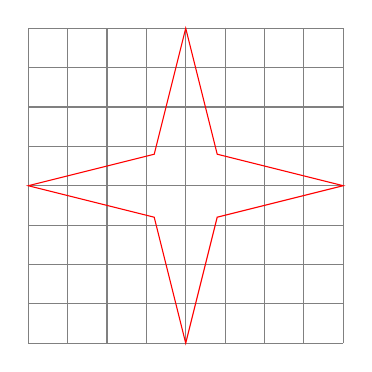
\begin{tikzpicture}[scale=2]
          \draw[step=0.25cm,color=gray] (-1,-1) grid (1,1);
          \draw[color=red] (1,0) -- (0.2,0.2) -- (0,1) -- (-0.2,0.2) -- (-1,0)
          -- (-0.2,-0.2) -- (0,-1) -- (0.2,-0.2) -- cycle;
        \end{tikzpicture}
        \caption{A figure caption}
      \end{figure}
    \end{column}
  \end{columns}

\end{frame}



% ====================
% References
% ====================

\begin{frame}[allowframebreaks]{References}
\printbibliography 
\end{frame}

% ====================
% Appendix
% ====================
\appendix
\appendixbegin
\begin{frame}{Appendix A}

Hi, I am an appendix

\end{frame}

\appendixend

\end{document}

